%%%%%%%% ICML 2019 EXAMPLE LATEX SUBMISSION FILE %%%%%%%%%%%%%%%%%

\documentclass{article}

% Recommended, but optional, packages for figures and better typesetting:
\usepackage{microtype}
\usepackage{graphicx}
\usepackage{subfigure}
\usepackage{booktabs} % for professional tables

% hyperref makes hyperlinks in the resulting PDF.
% If your build breaks (sometimes temporarily if a hyperlink spans a page)
% please comment out the following usepackage line and replace
% \usepackage{icml2019} with \usepackage[nohyperref]{icml2019} above.
\usepackage{hyperref}

% Attempt to make hyperref and algorithmic work together better:
\newcommand{\theHalgorithm}{\arabic{algorithm}}

% Use the following line for the initial blind version submitted for review:
%\usepackage{icml2021}

% If accepted, instead use the following line for the camera-ready submission:
\usepackage[accepted]{arxiv}

% The \icmltitle you define below is probably too long as a header.
% Therefore, a short form for the running title is supplied here:
\icmltitlerunning{Rethinking Neural Operations for Diverse Tasks}

\usepackage{amsmath,amssymb,amsthm}
\usepackage[ruled,vlined]{algorithm2e}
\usepackage[utf8]{inputenc}

% MATH ENVIRONMENTS
\newtheorem{Def}{Definition}[section]
\newtheorem{Thm}{Theorem}[section]
\newtheorem{Lem}{Lemma}[section]
\newtheorem{Cor}{Corollary}[section]
\newtheorem{Clm}{Claim}[section]
\newtheorem{Prp}{Proposition}[section]
\newtheorem{Asu}{Assumption}[section]
\newtheorem{Set}{Setting}[section]
\newtheorem{Rem}{Remark}[section]

% MATH OPERATORS
\DeclareMathOperator*{\argmin}{arg\,min}
\DeclareMathOperator*{\argmax}{arg\,max}
\DeclareMathOperator{\Tr}{Tr}
\newcommand{\Proj}{\operatorname{Proj}}
\newcommand{\Poly}{\operatorname{Poly}}
\newcommand{\Unif}{\operatorname{Unif}}
\newcommand{\prox}{\operatorname{prox}}
\newcommand\XD{\mathbf{XD}}
\newcommand{\Ch}{\mathbf{O}}
\DeclareMathOperator{\diag}{\operatorname{diag}}
\DeclareMathOperator{\Op}{\operatorname{\bf Op}}
\DeclareMathOperator{\Real}{\operatorname{Real}}
\newcommand{\BigO}{\mathcal O}
\DeclareMathOperator{\Conv}{\operatorname{\bf Conv}}
\DeclareMathOperator{\Lin}{\operatorname{\bf Lin}}
\DeclareMathOperator{\Id}{\operatorname{\bf Id}}
\DeclareMathOperator{\Zero}{\operatorname{\bf Zero}}
\DeclareMathOperator{\MaxP}{\operatorname{\bf MaxPool}}
\DeclareMathOperator{\AvgP}{\operatorname{\bf AvgPool}}
\DeclareMathOperator{\DilC}{\operatorname{\bf DilatedConv}}
\newcommand{\Update}{\texttt{Update}}
\newcommand{\Search}{\mathcal S}
\newcommand{\DARTS}{\mathbf{DARTS}}

% MATH SYMBOLS
\newcommand{\A}{\mathcal A}
\newcommand{\B}{\mathcal B}
\newcommand{\C}{\mathbb C}
\newcommand{\D}{\mathcal D}
\newcommand{\E}{\mathbb E}
\newcommand{\F}{\mathcal F}
\newcommand{\G}{\mathcal G}
\newcommand{\K}{\mathcal K}
\newcommand{\N}{\mathbb N}
\newcommand{\Q}{\mathcal Q}
\newcommand{\R}{\mathbb R}
\newcommand{\V}{\mathbb V}
\newcommand{\W}{\mathcal W}
\newcommand{\X}{\mathcal X}
\newcommand{\Y}{\mathcal Y}
\newcommand{\Z}{\mathbb Z}
\newcommand{\0}{\mathbf 0}
\newcommand{\1}{\mathbf 1}
\newcommand{\atr}{\mathfrak{a}}

% SMALL SQRT
\usepackage{scalerel,mathtools,color}
\let\svsqrt\sqrt
\newsavebox\Nsqrt
\def\sr#1{\ThisStyle{%
	\savebox\Nsqrt{\scalebox{.5}[1]{$\SavedStyle\svsqrt{\phantom{\cramped{#1#1}}}$}}%
	\ooalign{\usebox{\Nsqrt}\cr\kern.2pt\usebox{\Nsqrt}\cr\hfil$\SavedStyle\cramped{#1}$}}}
\def\pl{\texttt{+}}
\newcommand{\sd}{\scalebox{0.64}[1]{$\dots$}}

% BACKSLASH BOLDING
\usepackage{enumitem}
\usepackage{bm}
\def\*#1{\mathbf{#1}}

% TABLES
\usepackage{threeparttable,multirow}

% Commenting
%\newcommand\misha[1]{{\color{red}#1}}
%\newcommand\nick[1]{{\color{blue}#1}}

\usepackage{ilatex}
\usepackage{gridlayout}

\begin{document}

\twocolumn[
\icmltitle{
	Rethinking Neural Operations for Diverse Tasks
}

% It is OKAY to include author information, even for blind
% submissions: the style file will automatically remove it for you
% unless you've provided the [accepted] option to the icml2021
% package.

% List of affiliations: The first argument should be a (short)
% identifier you will use later to specify author affiliations
% Academic affiliations should list Department, University, City, Region, Country
% Industry affiliations should list Company, City, Region, Country

% You can specify symbols, otherwise they are numbered in order.
% Ideally, you should not use this facility. Affiliations will be numbered
% in order of appearance and this is the preferred way.
\icmlsetsymbol{equal}{*}

\begin{icmlauthorlist}
	\icmlauthor{Nicholas Roberts}{equal,cmu}
	\icmlauthor{Mikhail Khodak}{equal,cmu}
	\icmlauthor{Tri Dao}{stanford}
	\icmlauthor{Liam Li}{dai}
	\icmlauthor{Christopher R\'e}{stanford}
	\icmlauthor{Ameet Talwalkar}{cmu,dai}
\end{icmlauthorlist}

\icmlaffiliation{cmu}{Carnegie Mellon University}
\icmlaffiliation{stanford}{Stanford University}
\icmlaffiliation{dai}{Determined AI}

\icmlcorrespondingauthor{Nicholas Roberts}{\texttt{ncrobert@cs.cmu.edu}}
\icmlcorrespondingauthor{Mikhail Khodak}{\texttt{khodak@cmu.edu}}

% You may provide any keywords that you
% find helpful for describing your paper; these are used to populate
% the "keywords" metadata in the PDF but will not be shown in the document
\icmlkeywords{Machine Learning, ICML}

\vskip 0.3in
]

% this must go after the closing bracket ] following \twocolumn[ ...

% This command actually creates the footnote in the first column
% listing the affiliations and the copyright notice.
% The command takes one argument, which is text to display at the start of the footnote.
% The \icmlEqualContribution command is standard text for equal contribution.
% Remove it (just {}) if you do not need this facility.

%\printAffiliationsAndNotice{}  % leave blank if no need to mention equal contribution
\printAffiliationsAndNotice{\icmlEqualContribution} % otherwise use the standard text.

% !TEX root = main.tex

\begin{abstract}

	An important goal of neural architecture search (NAS) is to automate-away the design of neural networks on new tasks in under-explored domains. 
	Motivated by this broader vision for NAS, we study the problem of enabling users to discover the right neural operations given data from their specific domain.
	We introduce a search space of neural operations called XD-Operations that mimic the inductive bias of standard multi-channel convolutions while being much more expressive:
	we prove that XD-operations include many named operations across several application areas.
	Starting with any standard backbone network such as LeNet or ResNet, we show how to transform it into an architecture search space over XD-operations and how to traverse the space using a simple weight-sharing scheme.
	On a diverse set of applications---image classification, solving partial differential equations (PDEs), and sequence modeling---our approach consistently yields models with lower error than baseline networks and sometimes even lower error than expert-designed domain-specific approaches.
	
\end{abstract}
% !TEX root = main.tex

\section{Introduction}

Neural architecture search is often motivated by the \mbox{AutoML} vision of democratizing machine learning (ML) by reducing the need for expert deep net design, both on existing problems and in new domains.
While NAS research has seen rapid growth with developments such as weight-sharing \citep{pham2018enas} and ``NAS-benches" \citep{ying2019nasbench101,zela2020nasbench1shot1}, most efforts focus on search spaces that glue together established primitives for well-studied tasks like vision and text \citep{liu2019darts,li2019rsws,xu2020pcdarts,li2021gaea} or on deployment-time issues such as latency \citep{cai2020ofa}.

In this work, we revisit a broader vision for NAS, proposing to move towards much more general search spaces while still exploiting successful components of leading network topologies and efficient NAS methods.
To do so we focus exclusively on expanding the set of operations, which is usually fairly small;
for example, that of the well-studied DARTS space has cardinality eight and consists of a few types of convolution and pooling layers \citep{liu2019darts}.
The baseline approach for expanding this set---adding known operations one-by-one---scales poorly and will not result in new types of operations when faced with new types of data.

%Our core contribution is a re-imagining of NAS operation spaces inspired by {\em weight-sharing} \citep{pham2018enas}, a popular search approach in which a gradient algorithm optimizes a ``supernet" objective that interpolates the set of operations on each edge using a continuous relaxation.
%While most past work simply uses a convex combination of operations \citep{liu2019darts}, our search space is based upon an alternative continuous relaxation that exploits the fact that most of these operations return linear transforms diagonalized by the discrete Fourier transform (DFT).
%Replacing the DFT matrices in the diagonal decomposition by a more expressive family of efficient linear transforms known as {\em Kaleidoscope} or {\em K-matrices} \citep{dao2020kaleidoscope} yields the set of {\bf Expressive Diagonalization (XD) Operations}, which comprise a large search space containing various types of grid-based convolutions and pooling, permutations, certain kinds of graph convolutions, the Fourier Neural Operator (FNO) from the PDE literature \citep{li2021fno}, and infinitely many more.

Our core contribution is a re-imagining of NAS operation spaces that drastically expands them in a principled fashion to include both standard operations as well as a wide range of new ones. 
To do so we exploit the fact that most standard operations used in modern NAS return linear transforms diagonalized by the discrete Fourier transform (DFT). Replacing the DFT matrices in the diagonal decomposition by a more expressive family of efficient linear transforms known as {\em Kaleidoscope} or {\em K-matrices} \citep{dao2020kaleidoscope} yields the set of {\bf Expressive Diagonalization (XD) Operations}, which comprise a large search space containing various types of grid-based convolutions and pooling, permutations, certain kinds of graph convolutions, the Fourier Neural Operator (FNO) from the PDE literature \citep{li2021fno}, and infinitely many more.
This broad expressivity reflects the key insight of our work:
that many of the most important neural operations in ML consist of multiple channels that apply weights $\*w$ to inputs $\*x$ by computing
\begin{equation}
\*K\diag(\*L\*w)\*M\*x
\end{equation}
where the matrices $\*K$, $\*L$, and $\*M$ are {\em efficient} (to represent and apply) and shared across channels.
%By design, all XD-operations are also computationally efficient and have small description length.

\begin{figure*}[ht!]
	\centering
		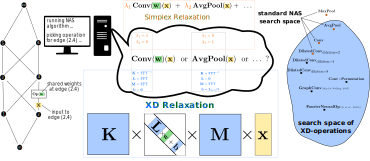
\includegraphics[width=\linewidth]{figures/main/main.pdf}
	\caption{\label{fig:main}
		Diagram of our search space in the single-channel case depicting a NAS method picking an operation to assign to an edge in a backbone network (left).
		Instead of choosing from a discrete search space, we use a relaxation based on the convolution's diagonalization by the discrete Fourier transform in which the DFT matrices are replaced by K-matrices \citep{dao2020kaleidoscope} $\*K$, $\*L$, and $\*M$ (middle);
		these comprise the main architecture parameters of our new search space over Expressive Diagonalization (XD) operations.
		This space contains most operations considered in past NAS research as well as many other important operations in a variety of domains (right).
	}
\end{figure*}

We leverage XD-operations to take critical steps towards a broader NAS that enables the discovery of good design patterns with limited human specification from data in under-explored domains.
To do so we develop a simple procedure which transforms a backbone network into an architecture search space by replacing its operations with XD-operations.
This space is then searched using a simple weight-sharing algorithm that needs only a small amount of tuning to find effective operations.
Finally, we demonstrate the effectiveness of this approach and the need for such a broader class of operations in a series of applications.  
\begin{itemize}[leftmargin=*,topsep=-1pt,noitemsep]\setlength\itemsep{2pt}
	\item We first demonstrate the fragility of NAS operation spaces---and thus the need for XD-operations---with a simple experiment using CIFAR-10.
	While searching over XD-operations and DARTS operations yields comparable performance using the LeNet and ResNet-20 backbones on the original data, models found using XD-operations are 15\% more accurate when the images are permuted.
	In this setting, we even exceed a state-of-the-art NAS algorithm over the DARTS search space by 7\% while using a much smaller model.
	\item We study the problem of solving PDEs, applying XD-operations using a simple convolutional backbone.
	We substantially outperform convolutions and even achieve lower error than the custom-designed, state-of-the-art Fourier Neural Operators (FNOs) of \citet{li2021fno} across three problems with different dimensionalities (Burgers' equation, Darcy Flow, and Navier-Stokes) when comparing to FNOs of the same dimensionality.
	Our method also maintains consistent performance across different resolutions, a major stated advantage of FNOs over previous methods. 
	\item We study four problems in sequence modeling using temporal convolutional networks (TCNs) \cite{bai2018tcn} as backbones.
	By substituting XD-operations we exceed this strong baseline, itself usually better than classical recurrent nets such as LSTMs, on all tasks, including by four perplexity points on word-level Penn Treebank.
\end{itemize}

Code to reproduce these results is available here: \url{https://github.com/nick11roberts/XD}.


%
%\begin{algorithm}[!h]
%	\DontPrintSemicolon
%	\KwIn{input to algorithm}
%	\For{iteration}{
%		do something \tcp*{comment}
%	}
%	\caption{\label{alg:example}
%		algorithm description
%	}
%\end{algorithm}
%
%\begin{table}[!h]
%	\centering
%	\begin{threeparttable}
%		\begin{tabular}{lccccccc}
%			\hline
%			& & \multicolumn{2}{c}{heading}& heading  & heading & heading & heading \\  
%			heading & heading & subheading & subheading & subheading & subheading & subheading & subheading \\
%			\hline
%			section 1$^\ast$ & - & - & - & - & - & - & - \\
%			\hline
%			section 2$^\dagger$ & - & - & - & - & - & - & - \\
%			\hline
%		\end{tabular}
%		\begin{tablenotes}
%			\item[$\ast$] table note 1
%			\item[$\dagger$] table note 2
%		\end{tablenotes}
%		\caption{\label{tab:example}
%			table description
%		}
%	\end{threeparttable}
%\end{table}
% !TEX root = main.tex

\subsection{Related Work}

AutoML is a well-studied area, with most work focusing on fairly small hyperparameter spaces \citep{bergstra2012rs,li2018hyperband} or on NAS \citep{elsken2019nas}.
Most NAS operation spaces only contain a few specific operations such as convolutions \citep{liu2019darts,zela2020nasbench1shot1,dong2020nasbench201};
even when expanded to include many filter sizes \citep{mei2020atomnas}, such search spaces may not be useful for domains where convolutions are ineffective.
Applications of NAS outside vision have largely followed the same pattern of combining human-designed primitives \citep{nekrasov2019nas,wang2020textnas}. 
On the other extreme, \citet{real2020automlzero} demonstrated the possibility of evolving all aspects of ML---not just the model but also its learning algorithm---from scratch.
We seek to establish a middle ground with large and domain-agnostic search spaces that still allow the application of well-tested learning algorithms, e.g. stochastic gradient descent (SGD).
%In the latter case, it has been observed that the search spaces are still ``easy" in the sense that random architectures do reasonably well \citep{elsken2019nas,li2019rsws}.
%Our main contribution is a family of search spaces generalizing convolutions \citep{lecun1999lenet}.

Several papers have generalized the DFT to replace layers in deep networks \citep{dao2019butterfly,alizadeh2020butterfly,ailon2020butterfly}, including the one whose K-matrices we apply \cite{dao2020kaleidoscope}.
These works focus on replacing {\em linear} layers in deep nets to speed up or add structure to models while {\em reducing} expressivity.
In contrast, we can replace {\em convolutions} and other types of layers while {\em increasing} expressivity by extending their diagonalization using K-matrices.
As discussed in Section~\ref{sec:relax}, using K-matrices to do this directly is inefficient for input dimension $>1$.

%Beyond NAS, recent work by \citet{zhou2021symmetries} uses a meta-learning framing \citep{thrun1998ltl} to study how to learn more general types of symmetries---beyond simply translational---from multi-task data.
%This transfer-based setup allows a clear formalization of learning such equivariances, though unlike NAS, it is not applicable to single-task settings.
%In addition, their technical approach does not generalize 2d convolutions due to computational intractability, while our XD-operations are indeed able to do so.

%Recently, \citet{neyshabur2020convolutions} showed that sparsity-inducing optimization can train fully connected nets that match the performance of convolutional networks and in the process the weights learn local connectivity patterns.
%However, none of these papers return parameterizable operations from a formally defined search space.
% !TEX root = main.tex

\section{The Expressive Diagonalization Relaxation}\label{sec:relax}

In this section we overview our main contribution:
a large, general search space of neural operations.
Formally, we view a neural architecture as a {\em parameterizable} object---a mapping from model weights to functions---that can be described by a {\em labeled} directed acyclic graph (DAG) $\G(V,E)$.
Each edge in $E$ has the form $(u,v,\Op)$, where $u,v\in V$ are nodes and $\Op$ is an operation that can be parameterized to define some transformation of the representation at node $u$;
node $v$ aggregates the outputs of its incoming edges to construct a new representation.
For example, the popular ResNet architecture \citep{he2016resnet} has many nodes $v$ with two incoming edges, one labeled by the convolution operation $\Conv$ and one labeled by the identity (skip-connect) operation $\Id$, whose outputs it sums and passes to two outgoing edges with the same labels.
Each architecture DAG has a source node into which we pass input data and an output node that returns a prediction or score.

Neural architecture search is the problem of automatically selecting which operation to use at each edge of $\G$ in order to optimize some objective.\footnote{It is often defined as selecting both operations and a graph topology \citep{zoph2018nas}, but if the set of operations contains the zero-operation $\Zero$ then the former subsumes the latter.}
For each edge $e\in E$ a NAS algorithm must pick one element of a {\em search space} $\Search=\{\Op_a\vert a\in\A\}$ of operations specified by architecture parameters $a\in\A$ to assign to $e$;
in past work, $\A$ has usually indexed a small set of operations.
As an example, we will refer to a variant\footnote{For memory-efficiency, all convolutions in the original DARTS search space are separable \citep{liu2019darts}.} of the DARTS search space in which $\A_\DARTS=\{1,\dots,8\}$, with each operation $\DARTS_a\in\Search_\DARTS$ being one of $\Zero$, $\Id$, $\MaxP_{3\times 3}$, $\AvgP_{3\times 3}$, $\Conv_{3\times 3\textrm{ or }5\times 5}$, or $\DilC_{3\times 3,2\textrm{ or }5\times 5,2}$ \citep{liu2019darts}.

Our main contribution is a novel family of operations that comprise a search space containing almost all these operations, in addition to many others that have been found useful on different types of data.
The starting point of our construction of these XD-operations is the simple observation that all the operations $\Op\in\Search_\DARTS$ listed above except $\MaxP_{3\times3}$ are {\em linear}, i.e.
for any model weights $\*w$ there exists a matrix $\*A_{\*w}$ such that for all inputs $\*x$ we have $\Op(\*w)(\*x)=\*A_{\*w}\*x$.
More specifically, all seven of them return convolutions:
to see this note that $\Zero$, $\Id$, and $\AvgP_{3\times3}$ each apply a convolution with filter $\0_{1\times1}$, $\1_{1\times1}$, and $\1_{3\times3}/9$, respectively.
This means that most of the operations in the DARTS search space---which is representative of NAS operation spaces in computer vision---share the convolution's diagonalization by the discrete Fourier transform (DFT).
Formally, if $\*A_{\*w}\in\R^{n^2\times n^2}$ is the matrix representing a 2d convolution with filter $\*w\in\R^{\*k}$ of kernel size $\*k\in[n]^2$, then for any 2d input $\*x\in\R^{n^2}$ we have
\begin{equation}\label{eq:fourier}
\Conv(\*w)(\*x)=\*A_{\*w}\*x=\*F^{-1}\diag\left(\*F\underline{\*w}\right)\*F\*x
\end{equation}
Here $[n]=\{1,\dots,n\}$, $\diag(\*z)$ denotes the diagonal matrix with nonzero entries $\*z$, $\underline{\*w}\in\R^{n^2}$ is an appropriate zero-padding of $\*w\in\R^{\*k}$, and $\*F\in\C^{n^2\times n^2}$ is the 2d DFT (a Kronecker product of two 1d DFTs).

This diagonalization explicates both the computational and representational efficiency of the DARTS operations, as both the DFT and its inverse can be applied in time $\BigO(n\log n)$ and represented with $\BigO(n\log n)$ bits.
It also suggests a natural way to dramatically expand the operation space while preserving these efficiencies:
simply replace the Fourier matrices $\*F$ and $\*F^{-1}$ in \eqref{eq:fourier} by a more general family of efficient matrices.
Doing so yields the single-channel version of our {\em expressive diagonalization} (XD) operations:
\begin{equation}\label{eq:xd1}
\XD_\alpha^\1(\*w)(\*x)=\Real\left(\*K\diag\left(\*L\underline{\*w}\right)\*M\*x\right)
\end{equation}
Here the architecture parameter $\alpha=(\*K,\*L,\*M)$ determines the exact matrices used to replace $\*F$ and $\*F^{-1}$ in Equation~\ref{eq:fourier}.

The main remaining question is the family of efficient matrices to use, i.e. the domain of the architecture parameters $\*K$, $\*L$, and $\*M$.
For this we turn to the Kaleidoscope matrices, or {\em K-matrices}, of \citet{dao2020kaleidoscope}, which generalize $\*F$ and $\*F^{-1}$ to include all computationally efficient linear transforms with short description length.
This includes important examples, such as sparse matrices and permutations, that add significant expressivity to the DFT.
To obtain this general family, K-matrices allow the DFT's butterfly factors---matrices whose products yield its efficient implementation---to take on different values.
While a detailed construction of K-matrices can be found in the original paper, we need only the following useful properties: 
they are as (asymptotically) efficient to apply and represent as DFTs, they are differentiable and can thus be updated using gradient-based methods, and they can be composed (made ``deeper") to make more expressive K-matrices.

Specifying that $\*K$, $\*L$, and $\*M$ in Equation~\ref{eq:xd1} are K-matrices largely completes our core contribution:
a new search space $\Search_\XD$ of XD-operations with K-matrix architecture parameters.
We give a full multi-channel formalization in $N$ dimensions, as well as an overview of its expressivity, in Section~\ref{sec:xd}.
First, we note some key aspects of this new search space:
\begin{itemize}[leftmargin=*,topsep=-1pt,noitemsep]\setlength\itemsep{2pt}
	\item{\bf Complexity:} the function $\XD_\alpha^\1$ requires three K-matrices and $\BigO(1)$ filter weights to represent, which implies description length $\BigO(n\log n)$;
	this is larger than a regular convolution (which has no architecture parameters) but is not quadratic in the input size like a linear layer.
	Applying $\XD_\alpha^\1$ requires multiplication by three K-matrices, yielding a per-channel time complexity of $\BigO(n\log n)$. 
	This matches the efficiency of convolutions.
	\item{\bf Initialization:} a crucial advantage of XD-operations is that we can initialize or {\em warm-start} search using operations with known constructions.
	In particular, since we can recover convolutions \eqref{eq:fourier} by setting architecture parameters $\*K=\*F^{-1}$, $\*L=\*F$, and $\*M=\*F$ in Equation~\ref{eq:xd1}, we can always start search with any convolutional backbone network.
	We use this extensively in experiments.
	\item{\bf K-matrices:} as they contain all efficient linear transforms, K-matrices can represent all functions returned by XD-operations, including convolutions.
	However, if both the input dimension $N$ and filter size are $>1$, as in most applications, then the only known way is to apply K-matrices directly to flattened inputs $\*x\in\R^{n^N}$, yielding much worse description length $\BigO(n^N\log n)$.
	In contrast, as detailed in Section~\ref{subsec:xdmc} our diagonalization approach allows the use of Kronecker products to apply DFTs to each dimension separately, yielding description length $\BigO(n\log n)$.
	It is thus the first (and in some sense, ``right") method to use such matrices as replacements for convolutions.
	Furthermore, diagonalization allows us to separate model weights $\*w$ from architecture parameters $\alpha$, letting the former vary across channels while fixing the latter.
\end{itemize}

Finally, we address the fact that the architecture parameters of $\Search_\XD$ are continuous, not discrete, contrasting with much of the NAS literature.
This can be viewed as a natural extension of the weight-sharing paradigm \citep{pham2018enas}, in which continuous relaxation enables updating architecture parameters with gradient methods.
For example, many algorithms traverse the relaxed DARTS search space 
$\tilde\Search_\DARTS=\left\{\sum_{i=1}^8\lambda_i\DARTS_i\vert\lambda_i\ge0,\sum_{i=1}^8\lambda_i=1\right\}$, defined via DARTS operations $\DARTS_i\in\Search_\DARTS$ and architecture parameters $\lambda_i$ in the 8-simplex;
most search spaces then requires discretizing after search via a rounding procedure that maps from the simplex to $\A_\DARTS$.

Our XD-relaxation avoids the poor scaling of the simplex relaxation when operations are added one-by-one.
In particular, the per-iteration cost of many NAS algorithms increases linearly with operation count \citep{liu2019darts} while the number of iterations of state-of-the-art methods increases logarithmically in the same \citep{li2021gaea}.
In contrast, $\Search_\XD$ contains numerous useful operations while taking roughly as long to search on CIFAR-10 as $\tilde\Search_\DARTS$.

%In the remainder of this section, we first formalize parameterizable operations, which will be useful in both our construction of XD-operations and in our analysis of their expressivity.
%Then we specify our new search space and describe several useful properties.
%Finally, we conclude by analyzing the expressivity of XD-operations by providing numerous examples of important named neural operations that they contain.
%This last step is critical because it enables us to initialize search using the operations specified in many backbones across a variety of applications.

%Finally, we note three properties that parameterizable operations on $\X=\R^{n\times n}$ can have that may be desirable from a computational or sample efficiency view:
%
%\begin{Def}\label{def:eff}
%	A parameterizable operation $\Op$ over parameter space $\W$ is {\bf computationally efficient} if given arbitrary $\*w\in\W$ and $\*x\in\R^n$ we can compute $\Op(\*w)(\*x)$ to arbitrary precision in time $\BigO(n\log n)$.
%\end{Def}
%
%\begin{Def}\label{def:dl}
%	A parameterizable operation $\Op$ over parameter space $\W$ has {\bf short description length} if every parameterized function $\Op(\*w):\R^n\mapsto\R^n$ can be represented to arbitrary precision with $\BigO(n\log n)$ bits.
%\end{Def}
%
%\begin{Def}\label{def:lin}
%	A parameterizable operation $\Op$ over parameter space $\W$ is {\bf linear} if for every $\*w\in\W$ there exists $\*A_{\*w}\in\R^{n\times n}$ such that $\Op(\*w)=\Lin(\*A_{\*w})$.
%\end{Def}
%
%An example of an operation that satisfies all three properties is the convolution operator.
%A simple operation that does not have short description length and is not efficient is the linear operation, which requires a number of parameters and a computation time that are both quadratic in the number of inputs.
%For an example of an operation that is not linear consider the multi-head self-attention mechanism in Transformer architectures \citep{vaswani2017attention}.

\section{XD-Operations and Their Expressivity}\label{sec:xd}

Here we formalize XD-operations and discuss what operations they can express.
To do so, we first define operations:
\begin{Def}\label{def:po}
	A {\bf parameterizable operation} is a mapping $\Op:\W\mapsto\F$ from parameter space $\W$ to a space $\F=\{\Op(\*w):\X\mapsto\Y\vert\*w\in\W\}$ of {\bf parameterized functions} from input space $\X$ to output space $\Y$.
	A {\bf search space} is a set of operations with the same $\W$, $\X$, and $\Y$.
\end{Def}

For example, if $\X=\Y=\R^n$ and $\W=\R^{n\times n}$ then each $\*W\in\W$ defines a parameterized linear layer that for each $\*x\in\X$ returns $\Lin(\*W)(\*x)=\*W\*x$.
Here $\Lin$ is the parameterizable operation and for each $\*W$ the linear map $\Lin(\*W)$ is the parameterized function.

From Definition~\ref{def:po}, we say a search space can {\em express} a specific operation if it contains it.
Crucially, the ability of a parameterizable operation $\Op_1$ to express a parameterized function $\Op_2(\*w)$ output from another operation $\Op_2$ given the right set of weights $\*w$ does {\em not} imply that a search space containing $\Op_1$ can express $\Op_2$.
For example, $\Lin(\*I_n)=\Id(\*W)~\forall~\*W\in\R^{n\times n}$ but $\Lin(\*W)\ne\Id(\*W)~\forall~\*W\ne\*I_n$, so a search space containing the linear operation $\Lin$ cannot express the skip-connection $\Id$, despite the fact that $\Lin$ can be parameterized to compute the identity.

%As exemplified by the DARTS search space $\Search_\DARTS$, modern search spaces generally contain a fairly limited number of operations.
%Of these operations only convolutions use their model weights, and they may not always be the right choice in non-vision domains.
%Our goal is instead to construct a significantly larger search space that contains effective operations for many tasks.
%Still, because convolutions satisfy the three desirable properties above, are used as baselines in many fields, and share a diagonalization with basic pooling operations including $\AvgP$ and $\Id$, our construction is designed as an extension of them.
%In particular, we start with the diagonalization of the matrix $\*A_{\*w}\in\R^{n^N\times n^N}$ representing a convolution with filter $\*w\in\R^{\*k}$ of kernel size $\*k\in[n]^N$ by the $N$-dimensional discrete Fourier Transform (DFT) $\*F\in\C^{n^N\times n^N}$ (a Kronecker product of $N$ 1d DFTs):
%\begin{equation}\label{eq:fourier}
%\Conv(\*w)(\*x)=\*A_{\*w}\*x=\*F^{-1}\diag(\*F\underline{\*w})\*F\*x
%\end{equation}
%Here $\*x$ is any element of $\R^{n^N}$, $[n]=\{1,\dots,n\}$, $\diag(\*z)$ denotes the diagonal matrix with nonzero entries $\*z$, and $\underline{\*w}\in\R^{n^N}$ is an appropriate zero-padding of $\*w\in\R^{\*k}$.
%
%The convolution's diagonalization explicates both its computational and representational efficiency, as both the DFT and its inverse can be applied in time $\BigO(n\log n)$ and represented with $\BigO(n\log n)$ bits.
%Starting from the butterfly diagrams that represent the construction of the DFT as a product of small factor matrices, \citet{dao2020kaleidoscope} introduced Kaleidoscope matrices, or {\em K-matrices}, which generalize $\*F$ and $\*F^{-1}$ to include all computationally efficient linear transforms with short description length.
%This includes important examples, such as sparse matrices and permutations, that add significant expressivity to the DFT.
%While a detailed construction of K-matrices can be found in the original paper, we need only the above efficiency properties, the fact that we can update the K-matrix representation using gradient-based methods, and the ability to compose multiple K-matrices into deeper ones;
%in particular we say that a K-matrix has depth-$d$ if it is a product of $d$ depth-1 K-matrices.

\subsection{Formalizing Multi-Channel XD-Operations}\label{subsec:xdmc}

Recall the single-channel XD-operation $\XD_\alpha^\1$ in Equation~\ref{eq:xd1}, which is parameterized by a three-matrix architecture parameter $\alpha=(\*K,\*L,\*M)$.
In the general case of input dimension $N\ge1$, every matrix $\*B\in\alpha$ is a Kronecker product of $N$ $K$-matrices of depth $\*d\in\Z_+^3$, i.e. $\*B=\bigotimes_{i=1}^N\*B_i$ for K-matrices $\*B_i\in\C^{n\times n}$ of depth $\*d_{[1]}$, $\*d_{[2]}$, or $\*d_{[3]}$ for $\*B=\*K$, $\*L$, or $\*M$, respectively.\footnote{A depth-$d$ K-matrix is a product of $d$ depth-1 K-matrices.}
Roughly speaking, $\XD_\alpha^\1$ can express a set of linear operations that can be diagonalized by K-matrices and are thus efficient to compute and represent, such as convolutions (recall that we recover the diagonalization of $\Conv(\*w)$ in Equation~\ref{eq:fourier} by setting $\*K$, $\*L$, and $\*M$ appropriately in Equation~\ref{eq:xd1}).
However, $\XD_\alpha^\1$ cannot represent efficient {\em parameter-free} operations such as skip-connections and average-pooling, both common in NAS.
In particular, the only way to force the operation to ignore the model weights $\*w$ is to set one of the K-matrices to zero, producing the zero-operation.
We can avoid this by adding a bias vector $\*b\in\C^{n^N}$ as an architecture parameter, producing the {\em biased} single-channel XD-operation:
\begin{equation}\label{eq:biased}
\XD_{\alpha,\*b}^\1(\*w)(\*x)=\Real\left(\*K\diag(\*L\underline{\*w}+\*b)\*M\*x\right)
\end{equation}
Doing this allow us to define skip-connections (set $\*K$ and $\*M$ to the identity, $\*L$ to the zero matrix, and $\*b=\1_{n^N}$) and average-pooling (set $\*K=\*F^{-1}$, $\*L=\0_{n^N\times n^N}$, $\*M=\*F$, and $\*b$ to be $\*F$ multiplied by the appropriate pooling filter).

Our last step is to use $\XD_{\alpha,\*b}^\1$ to construct multi-channel ``layers" that pass multiple input features through multiple channels and re-combine them as multiple output features.
This follows the primary way of using convolutions in deep nets, which is to apply multiple convolutions with different filters to multiple inputs.
The key insight here is that we will share the same parameterizable operation (specified by $\alpha$ and $\*b$) across all channels, just as in convolutional layers.
\begin{Def}\label{def:xd}
	Let $a=(\alpha,\*b,\*C)$ be an architecture parameter where $\alpha=(\*K,\*L,\*M)$ is a triple of Kronecker products of $N$ K-matrices with depths $\*d\in\Z_+^3$, $\*b\in\C^{n^N}$ is a bias term, and $\*C\in\C^{c\times c}$ is a matrix of channel gates.\footnote{For simplicity we formalize the case where all $N$ dimensions have the same input size $n$ and there is an identical number $c$ of input and output channels; both are straightforward to extend.}
	The {\bf XD-operation} $\XD_a$ of depth $\*d$ specified by $a$ is a parameterizable operation on parameter space $\W=\R^{c\times c\times\*k}$ consisting of $c^2$ filters of size $\*k\in[n]^N$ that outputs parameterized functions on $\X=\R^{c\times n^N}$ mapping every $\*x\in\X$ to\vspace{-5pt}
	\begin{equation}
	\XD_a(\*w)(\*x)=
	\begin{pmatrix}
	\sum\limits_{j=1}^c\*C_{[1,j]}\XD_{\alpha,\*b}^\1(\*w_{[1,j]})(\*x_{[j]})\\
	\vdots\\
	\sum\limits_{j=1}^c\*C_{[c,j]}\XD_{\alpha,\*b}^\1(\*w_{[c,j]})(\*x_{[j]})
	\end{pmatrix}
	\end{equation}
	We use $\Search_\XD$ to describe the set of such operations.
\end{Def}
The parameter $\*C$ allows interpolation between all-to-all layers ($\*C=\1_{c\times c}$), e.g. multi-channel convolutions, and layers where each channel is connected to one other channel ($\*C=\*I_c$), as in skip-connections and average-pooling.

We conclude our construction by discussing two properties:
%In particular, note that all XD-operations satisfy the properties in Definitions~\ref{def:eff},~\ref{def:dl}, and~\ref{def:lin}.
\begin{itemize}[leftmargin=*,topsep=-1pt,noitemsep]\setlength\itemsep{2pt}
	\item{\bf Kernel size:} the weight-space available to an XD-operation is $\R^{c\times c\times n^N}$; however, since we will initialize search with existing backbone nets, we will use zero-padding to have the same weight space $\R^{c\times c\times k^N}$ as the convolutions with filter size $k\le n$ that they replace.
	This preserves the number of weights but also means that if the backbone has $3\times3$ filters our search space will {\em not} contain $5\times5$ convolutions.
	Experimentally, we find that relaxing the constraint to allow this does not significantly affect results on image tasks, so we do not do so in subsequent applications to avoid increasing the weight count.
	\item{\bf Depth:} an XD-operation's depth is a triple describing the depths of its K-matrices $\*K$, $\*L$, and $\*M$.
	Increasing depth trades off efficiency for expressivity;
	for example, in the next section we describe operations that we can show are contained in $\Search_\XD$ if $\*L$ or $\*M$ have depth $>1$.
	By default we will set the depth to be the minimum needed to initialize search with the operation used by the backbone.
\end{itemize}


\subsection{Expressivity of XD-Operations}\label{subsec:express}

%\begin{table*}[!t]
%	\centering
%	\begin{threeparttable}
%		\begin{tabular}{ccrccccc}
%			\hline
%			{\bf Search space} & \multicolumn{2}{c}{Operation} & \multicolumn{5}{c}{Architecture setting, if distinct from $\Conv$} \\
%			weight space & \multicolumn{2}{c}{name} & $\*K$ & $\*L$ & $\*M$ & $\*b$ & $\*C$ \\
%			\hline
%			& \multicolumn{2}{l}{Convolution with filter size $n$ ($=\Conv$)} & $\*F^{-1}$&  $\*F$ & $\*F$ & $\0_n$ & $\1_{c\times c}$ \\
%			& \multicolumn{2}{l}{Convolution with filter size $k\in[n]$} & & $\*F\diag(\underline{\1_k})$ \\
%			$\{\XD_a\}$ & \multicolumn{2}{l}{$^\dagger$Dilated conv. with filter size $k$, dilation $s>1$} & & $\*F\diag(\underline{\*a_{k,s}})$ \\
%			& \multicolumn{2}{l}{$^\ddagger$Grouped conv. with filter size $k$, partition $g$ of $[c]$} & & $\*F\diag(\underline{\1_k})$ & & & $\*B_g$ \\
%			$\W=\R^{c\times c\times n}$ & \multicolumn{2}{l}{$^\ast$Multiplication by a fixed K-matrix $\*A\in\C^{n\times n}$} & & $\0_{n\times n}$ & $\*F\*A$ & $\*1_n$ & $\*I_c$ \\
%			& \multicolumn{2}{l}{$^\star$(Conv. with filter size $k$)\hspace{0.7mm}$\circ$\hspace{0.5mm}(Mult. by K-matrix $\*A$)} & & $\*F\diag(\underline{\1_k})$ & $\*F\*A$ \\
%			& \multicolumn{2}{l}{Average pooling with filter size $k\in[n]$} & & $\*0_{n\times n}$ & & $\frac1k\underline{\*F\1_k}$ & $\*I_c$ \\
%			\hline
%			$\{\XD_{a_1}\circ\XD_{a_2}\}$ & Depthwise-separable conv. & $\XD_{a_1}$: & & $\*F\diag(\underline{\1_1})$ & & & \\
%			$\W=(\R^{c\times c\times n})^2$ & with filter size $k$ & $\XD_{a_2}$: & & $\*F\diag(\underline{\1_k})$ & & & $\*I_c$ \\
%			\hline
%		\end{tabular}
%		\begin{tablenotes}\footnotesize
%			\item[$^\dagger$] $\*a_{k,s}\in\{0,1\}^{(k-1)s+1}$ is a vector with $s$ zeros between each of $k$ ones.
%			\item[$^\ddagger$] $\*B_g\in\{0,1\}^{c\times c}$ satisfies $\*B_g[i,j]=1\iff i$ and $j$ are in the same group in the partition $g$ of the set of channels $[c]$.
%			\item[$^\ast$] Includes skip-connections ($\*A=\*I_n$) and the zero-operation ($\*A=\0_{n\times n}$).
%			\item[$^\star$] Includes convolutions of permutations ($\*A$ is a permutation) and graph convolutions ($\*A$ is a modified adjacency matrix and $k=1$).
%		\end{tablenotes}
%		\caption{\label{tab:expressivity}
%			\normalsize
%			Summary of operations contained in a search space over XD-operations when the input/output spaces $\X$ and $\Y$ are 1d;
%			extending these results to $N$-dimensions is straightforward.
%			Note that to handle all the operation in a single search space we require $\XD$ to have depth $\*d\ge(1,1,d)$, where $d$ is one plus the depth of the K-matrix $\*A$.
%		}
%	\end{threeparttable}
%\end{table*}

Several papers have proposed replacing deep net layers with efficient linear transforms \cite{moczulski2015acdc,dao2020kaleidoscope};
there the question of expressivity comes down to the capacity of the linear transform used.
For example, multi-channel layers composed of a K-matrix in every channel can represent a different transform in each, thus allowing the output to be any combination of operations such as DFTs, permutations, and many more.
Our case is less straightforward since we care about expressivity of the search space, not of parameterized functions, and our approach is less-expressive {\em by design} as all channels share the K-matrices $\*K$, $\*L$, and $\*M$.
The latter can be thought of a useful inductive bias on NAS:
the set of XD-operations is still much broader than the set of convolutions, but the way in which model weights are applied is the same across all channels of a layer.

Expressivity results are a way to see if this bias is useful or constraining.
Here we summarize some important operations that we can show are XD-operations in the 1d case; 
these facts are proved in the appendix and are straightforward to extend to multi-dimensional inputs.
Formally, there exists $\*d\in\Z_+^3$ such that the set of XD-operations of depth $\*d$ over weights $\W=\R^{c\times c\times k}$ and inputs $\X=\R^n$ contains
\begin{enumerate}[leftmargin=*,topsep=-1pt,noitemsep]\setlength\itemsep{2pt}
	\item all convolutions with filter size $\le k$, dilation at most $\lfloor\frac{n-1}{k-1}\rfloor$, stride at most $n-1$, and arbitrary channel groups.
	\item all of $\Id$, $\Zero$, or $\AvgP_s$ for any $s\le n$.
	\item composing either of the above with multiplication of all input or output channels by a bounded-depth K-matrix.
\end{enumerate}
Note this does not account for {\em all} important XD-operations, e.g. we show in the appendix that they can also express Fourier Neural Operators \citep{li2021fno} with $\le\lfloor k/2\rfloor$ modes.
Still, the 2d-versions of the first two account for non-separable variants of most operations considered in past NAS work in computer vision, apart from the nonlinear $\MaxP$ \citep{ying2019nasbench101,dong2020nasbench201}.
Note that depthwise-separable convolutions {\em are} contained in the set of compositions of XD-operations.
The third item implies that XD-operations can express the basic and diffusion graph convolutions over fixed graphs \citep{kipf2017gcn,li2018dcrnn}:
both are point-wise convolutions composed with a sparse linear transform based on the adjacency matrix, which  K-matrices can represent efficiently.

Apart from understanding our search space, a chief motivation for these results is to enable initializing search using the operations of existing backbones.
As a concrete example used in Section~\ref{sec:seq}, consider dilated convolutions, which for $k>1$ apply filters of effective size $(k-1)d+1$ with nonzero entries separated by $d$ zeros.
One could hope to express the application of $\DilC_{k,d}$ to an input $\*x\in\R^n$ in the single-channel setting as $\*F^{-1}\diag(\*F\diag(\*p_{k,s})\underline{\*w})\*F\*x$, where $\*p_{s,k}\in\{0,1\}^n$ zeroes out appropriate entries of $\underline{\*w}$, but this requires filter size $(k-1)d+1>k$, increasing the number of model weights.
Instead, we can use a permutation $\*P_{k,s}\in\{0,1\}^{n\times n}$ to place the $k$ entries of $\underline{\*w}$ into dilated positions before applying the DFT:
\begin{equation}\label{eq:dilated}
	\DilC_{k,s}(\*w)(\*x)=\*F^{-1}\diag(\*F\*P_{k,s}\underline{\*w})\*F\*x
\end{equation}
As permutations are depth-2 K-matrices \citep{dao2020kaleidoscope}, we can express $\DilC_{k,s}$ with an XD-operation of depth $(1,3,1)$, with $\*K=\*F^{-1}$, $\*L=\*F\*P_{k,s}$, and $\*M=\*F$.
% !TEX root = main.tex

\section{Finding Good XD-Operations}\label{sec:chrysalis}

This section outlines a simple NAS procedure that we use to evaluate XD-operations.
Recall that a NAS method must find an architecture by assigning operations as labels to each edge $(u,v,\Op)$ of a computational graph.
We aim to simultaneously find good operation-edge assignments and model weights, a goal distinct from the classic {\em two-stage} NAS formulation, which finds assignments in an initial search phase before training the resulting architecture from scratch \citep{ying2019nasbench101}.
However, the use of weight-sharing \citep{pham2018enas} extends NAS to {\em one-shot} objectives where model weights and architecture parameters are jointly optimized.
Under weight-sharing, architecture parameters become regular weights in a larger ``supernet," adding flexibility by extending the hypothesis class \citep{li2021gaea}.

To assess XD-operations directly, rather than consider a general set of graphs we assume the user provides a starter network with existing edge labels $\Op_{u,v}$ as a backbone.
We transform this into a weight-sharing supernet by reparameterizing each operation $\Op_{u,v}$ as an XD-operation $\XD_{a_{u,v}}$ with architecture parameter $a_{u,v}$.
Then we apply gradient-based methods to simultaneously update both $a_{u,v}$ and the model weights $\*w_{u,v}$  associated with each edge as follows:
\begin{itemize}[leftmargin=*,topsep=-1pt,noitemsep]\setlength\itemsep{2pt}
	\item {\bf Architecture parameters} $a_{u,v}$ are initialized using the original operation used by the backbone by setting $\Op_{u,v}=\XD_{a_{u,v}}$;
	$a_{u,v}$ is then updated via SGD or Adam \citep{kingma2015adam}.
	We tune step-size, momentum, and the number of ``warmup" epochs: 
	initial epochs during which only model weights $\*w_{u,v}$ are updated.
	This can be viewed as a specialized step-size schedule.
	\item {\bf Model weights} $\*w_{u,v}$ are initialized and updated using the routine provided with the backbone model.
\end{itemize}
This allows us to take advantage of established topologies and optimizers while still searching for new operations.

\section{Application: Image Classification}


\begin{table}[!t]
	\centering
	\begin{threeparttable}
		\begin{tabular}{lccc}
			\hline
			{\bf Backbone} & & Permuted & Cost \\
			~~search space & CIFAR-10 & CIFAR-10$^\ast$ & (hours$^\dagger$) \\
			\hline
			{\bf LeNet} & $75.5\pm0.1$ & $43.7\pm0.5$ & 0.3 \\
			~~$\tilde\Search_\DARTS$ & $75.6\pm3.4$ & $47.7\pm1.0$ & 1.0 \\
			~~$\Search_\XD$ & $77.7\pm0.7$ & $63.0\pm1.0$ & 0.9 \\
			\hline
			{\bf ResNet-20} & $91.7\pm0.2$ & $58.6\pm0.7$ & 0.6 \\
			~~$\tilde\Search_\DARTS$ & $92.7\pm0.2$ & $58.0\pm1.0$ & 5.3 \\
			~~$\Search_\XD$ & $92.4\pm0.2$ & $73.5\pm1.6$ & 5.6 \\
			\hline
			DARTS Cell$^\ddagger$ & $96.0\pm0.2$ & $66.3\pm0.5$ & 28.6 \\
			\hline
		\end{tabular}
		\begin{tablenotes}\footnotesize
			\item[$\ast$] No data augmentation used in the permuted case.
			\item[$\dagger$] On a V100 GPU; time for DARTS Cell is training cost only.
			\item[$\ddagger$] Search using GAEA PC-DARTS \citep{li2021gaea}; training using ``base" routine from \citet{yang2020nas}.\vspace{-4pt}
		\end{tablenotes}
		\caption{\label{tab:cifar}
			Search space comparison on CIFAR-10.
			Validation accuracies reported as averages over three trials.\vspace{-4pt}
		}
	\end{threeparttable}
\end{table}

\begin{figure*}[!t]
	\centerline{\includegraphics[width=0.666\columnwidth]{figures/pde_1d.pdf}
		\includegraphics[width=0.666\columnwidth]{figures/pde_2d.pdf}
		\includegraphics[width=0.666\columnwidth]{figures/pde_2d_trace.pdf}\vspace{-12pt}
	}
	\caption{
		\textbf{(a)} and \textbf{(b)} Relative error on Burgers' equation and Darcy Flow across different resolutions, including all those considered by \citet{li2021fno}.
		\textbf{(c)} Training curves (dotted) and test curves (solid) on Darcy Flow, showing better generalization of XD-operations.}
	\label{fig:pde}
\end{figure*}

We start by applying the above procedure to image classification.
As we seek to apply NAS to diverse tasks beyond computer vision, we study only simple settings that demonstrate the need for XD-operations, in particular the LeNet \citep{lecun1999lenet} and ResNet \citep{he2016resnet} backbones applied to two datasets: 
CIFAR-10 \citep{krizhevsky2009cifar} and a variant where the rows and columns of all images are permuted.
Since convolutions are the ``right" operation for images, we expect the convolution-centric baselines below to do well on CIFAR-10.
On the other hand, as the ``right" operation on permuted data, at least in layer one, is an inverse permutation followed by convolution, here we may see a benefit of using XD-operations, which contain this operation (recall $\Search_\XD$ includes compositions of convolutions with multiplication by a K-matrix, e.g. a permutation).

We compare applying the Section~\ref{sec:chrysalis} algorithm to the set of XD-operations with two baselines:
a similar method applied to the relaxed set $\tilde\Search_\DARTS$ of DARTS operations from Section~\ref{sec:relax} and a two-stage state-of-the-art algorithm---GAEA PC-DARTS \citep{li2021gaea}---over the DARTS space \cite{liu2019darts}.
To optimize over $\tilde\Search_\DARTS$ we take an approach similar to the DARTS algorithm:
parameterize the simplex using a softmax and apply Adam.
We experiment with both a uniform initialization and one biased towards the backbone operation.
While both $\Search_\XD$ and $\Search_\DARTS$ contain LeNet's $\Conv_{5\times 5}$ layers and ResNet's $\Conv_{3\times 3}$ and $\Id$, for LeNet's $\MaxP_{3\times 3}$ layer we initialize with the closest operation in each.
For direct comparison, both search spaces employ weights with maximum filter size $5\times 5$ and for both we evaluate the shared weights rather than retraining after search (we find that the latter hurts the performance of $\tilde\Search_\DARTS$).
We set the XD-operations' depth to $\*d=\*3_3$ to express both the dilated convolutions in $\Search_\DARTS$ and convolutions composed with permutations.

In Table~\ref{tab:cifar}, we see that while both the relaxed DARTS space and XD-operations perform comparably on regular images, XD-operations achieve around 15\% better accuracy with both backbones when the images are permuted.\footnote{\citet{dao2020kaleidoscope} also investigate permuted CIFAR-10; they obtain higher accuracies with a larger backbone net and an auxiliary loss that encourages permutation-like K-matrices.}
There they even significantly outperform standard cell-based search, despite the latter's much more expensive and intensive training routine (600 epochs v. the 200 used for ResNet-20), much larger model size (2.3 million parameters v. 1.2 million), and higher performance on regular images.
These results show that to enable NAS on diverse data, we will need a search space that contains truly novel operations, not just combinations of existing ones.
In the remainder of the paper, we study more diverse and realistic tasks that show further evidence that $\Search_\XD$ is a strong candidate for this.

%\subsection{Transforming LeNet: An Illustrative Example}
%
%\begin{table}[!t]
%	\centering
%	\begin{threeparttable}
%		\begin{tabular}{lccc}
%			\hline
%			{\bf Backbone} & CIFAR & Permuted & CIFAR \\
%			~operation & 10 & CIFAR-10 & 100 \\
%			\hline
%			{\bf LeNet} & \\
%			~linear layer & \\
%			~K-matrix layer & \\
%			~XD (fixed random) & \\
%			~XD (from scratch) & \\
%			~~+~offline eval.$^\ast$ & \\
%			~XD (warm start) & \\
%			~~+~offline eval.$^\ast$ & \\
%			\hline
%			{\bf ResNet-20} & \\
%			~XD (from scratch) & \\
%			~~+~offline eval.$^\ast$ & \\
%			~XD (warm start) & \\
%			~~+~offline eval.$^\ast$ & \\
%			\hline
%		\end{tabular}
%		\begin{tablenotes}\footnotesize
%			\item[$\ast$] For CIFAR-100 we transfer operations found on CIFAR-10.
%		\end{tablenotes}
%		\caption{\label{tab:cifar}
%			\normalsize
%			Comparison of fixed and found operations on CIFAR data using the LeNet and ResNet-20 backbones.
%			All XD operations used have depth (3,3,3).
%		}
%	\end{threeparttable}
%\end{table}
%
%We start our investigation with CIFAR image classification \citep{krizhevsky2009cifar} and the variant where the rows and columns of each image are separately permuted.
%LeNet \citep{lecun1999lenet}, a network with two convolutional and two fully connected layers, is the first backbone we study;
%to convert it into a search space we simply replace the convolutions by XD-operations.
%We compare search over XD-operations to several non-convolutional baselines:
%linear layers, K-matrix layers (each convolution in each channel is replaced by a K-matrix), and fixed random XD-operations.
%Searching for XD-operations significantly outperforms all of these baselines, showing that the XD parameterization is a useful constraint on top of linear or K-matrix layers.
%
%We make a distinction in Table~\ref{tab:cifar} between ``from scratch" search, in which the K-matrices in XD-operations are initialized to be random orthonormal, and ``warm start" search, which is the approach described in the previous section of initializing XD-operations to match the backbone operations.
%The purpose of this is to investigate whether we can ``re-discover" convolutions (or the respective ``right" operation in other domains) without knowing about them;
%as shown in Table~\ref{tab:cifar}, while warm-starting with convolutions does do better on regular images, from-scratch search almost matches convolutions (i.e. the original backbone) on images and in fact does much better on permuted images.
%Another distinction we make is between evaluating the found operations using the shared weights, which we will be doing in all subsequent sections, and ``offline evaluation" that fixes the found operations but re-initializes and retrains the model weights;
%this is in-line with the common two-stage NAS approach.
%We find that offline evaluation performs worse but that the learned operations are still quite effective, including when they are found on CIFAR-10 and used on CIFAR-100.
%
%\subsection{Transforming ResNet: A Scaled-Up Example}
%
%Next we study the same datasets using the higher performance ResNet-20 architecture \citep{he2016resnet} as a backbone.
%While we are again able to find better operations than convolutions when using them to initialize search, starting from scratch performs much worse, even on permuted images.
%This is likely due to the need with this backbone to warmup search by not updating architecture parameters for the first quarter of the training epochs.
%Thus for subsequent applications we focus on the warm start approach without offline evaluation, although our experiments with LeNet suggest that the alternative is still a viable future direction.
%
%Note that we replace both convolutions and skip-connections in the ResNet backbone with XD-operations;
%this slightly increases the model weight count because XD-operations are by default parameterizable.
%The choice to do this does not significantly affect performance, and the found operation ignores its model weights (i.e. $\*L\approx\0$), so for simplicity and to preserve the number of model weights we only replace parameterizable operations in the applications below.
% !TEX root = main.tex

\section{Application: Solving PDEs}

\begin{table}[!t]
	\centering
	\begin{threeparttable}
		\begin{tabular}{lcc}
					\hline
					& $\nu=10^{-4}$ & $\nu=10^{-5}$ \\
					Method                     & $T=30$ & $T=20$  \\ 
					\hline
					%FNO-3D \citep{li2021fno}                &    0.1918    &    0.1893   \\
					%FNO-2D \citep{li2021fno}                &     {\bf 0.1559}   &   {\bf 0.1556}    \\
					%U-Net \citep{li2021fno}                &     0.2051   &    0.1982   \\
					%TF-Net \citep{li2021fno}                &     0.2253   &   0.2268    \\
					%ResNet \citep{li2021fno}                &    0.2871    &   0.2753    \\
					%\hline
					CNN-3d backbone                 &    0.325    &  0.278    \\
					FNO-3d (reproduced)                           &   0.182     &  0.177   \\
					{\bf CNN-3d backbone XD}  &     {\bf 0.172}  &  {\bf 0.168}     \\
					\hline
				\end{tabular}
%		\begin{tablenotes}\footnotesize
%			\item[$\ast$] No data augmentation used in the permuted case.
%			\item[$\dagger$] Training using ``base" routine from \citet{yang2020nas}.
%		\end{tablenotes}
		\caption{\label{tab:navierstokes}
			Relative test error on the 2d Navier-Stokes equations at two different settings of the viscosity $\nu$ and number of time steps $T$. 
			Best results in each setting are {\bf bolded}.
		}
	\end{threeparttable}
\end{table}

\begin{table*}[!t]
	\centering
	\begin{threeparttable}
		\begin{tabular}{lcccc}
			\hline
			& Permuted MNIST$^\ast$ & ~JSB Chorales~~ & ~~~~Nottingham~~~~ & ~~~Penn Treebank \\
			Method (source)  & (error) & (loss) & (loss) & (perplexity) \\
			\hline
			LSTM \citep{bai2018tcn} & 14.3 & 8.45 & 3.29 & 78.93 \\
			GRU \citep{bai2018tcn} & 12.7 & 8.43 & 3.46 & 92.48 \\
			RNN \citep{bai2018tcn} & 74.7 & 8.91 & 4.05 & 114.50 \\
			TCN backbone \citep{bai2018tcn} & 2.8 & 8.10 & 3.07 & 88.68 \\
			TrellisNet \citep{bai2019trellis} & 1.87 & - & - & {\bf 54.19} \\
			R-Transformer \citep{wang2020rtransformer} & - & - & {\bf 2.37} & 84.38 \\
			HiPPO-LegS \citep{gu2020hippo} & {\bf 1.7} & - & - & - \\
			\hline
			TCN backbone (reproduced) & $2.89\pm0.04$ & $8.17\pm0.01$ & $2.97\pm0.01$ & $88.49\pm0.31$ \\
			{\bf TCN backbone XD} (ours) & ${\bf 1.75\pm0.11}$ & ${\bf 8.07\pm0.02}$ & $2.81\pm0.05$ & $84.11\pm0.25$ \\
			\hline
		\end{tabular}
		\begin{tablenotes}\footnotesize
			\item[$\ast$] We use depth $\*d=(3,3,3)$ XD-operations for permutations;
			elsewhere we use $(1,3,1)$ to warm-start with dilated convolutions.\vspace{-4pt}
		\end{tablenotes}
		\caption{\label{tab:seq}
			XD-operations applied to TCNs compared to recent empirical results in sequence modeling.
			Our results are averages of three trials.
			Methods achieving within one deviation of the best performance are {\bf bolded}.
		}
	\end{threeparttable}
\end{table*}

As our first non-vision application, we consider the task of solving PDEs, an important application area of ML in the natural sciences \citep{li2015butterfly, li2018multidimensional, sirignano2018dgm}.
In our setup, data generated by classical PDE solvers is used to learn functions from some initial condition or setting to the corresponding PDE solution, with the goal of replacing the solver by a deep net forward pass;
the latter can be orders of magnitude faster.
Specifically, we evaluate using the setting of \citet{li2021fno}, whose Fourier Neural Operator is a recent method that significantly improves upon previous neural approaches, including baseline convolutional networks (CNNs).
The three PDEs they study are the Burgers' equation, Darcy Flow, and the 2d Navier-Stokes equations, which involve 1d, 2d, and 3d data, respectively.
The first two are studied across multiple resolutions, while the last one is studied at different viscosities.

%As a setup, we consider the same setting as that of \citet{li2021fno}, specifically the Burgers' equation, Darcy Flow, and the Navier-Stokes equations;
%as the data domain of these tasks is 1d, 2d, and 3d, respectively, this application also allows us to examine the performance of XD-operations across several dimensionalities. We follow the setup from \citet{li2021fno} and evaluate on the same 1d Burgers', 2d Darcy Flow, and 2d Navier-Stokes datasets used in their experiments. Per \citet{li2021fno}, the 2d Navier-Stokes problem involves 3d data which treats time as a third dimension. 

Our approach here will be to take a simple CNN backbone---the type a scientist might use in a first attempt at a solution---and replace all convolutions by XD-operations.
As a baseline, we hope to do better than this backbone;
ambitiously, we hope to compete with the custom-designed FNO.
The specific CNN we use is simply the FNO architecture of the appropriate dimension $N$ from \citet{li2021fno} but with all $N$-dimensional FNOs replaced by $N$-dimensional convolutions;
this performs similarly to their CNN baselines.
In all cases we only compare to the CNN backbone and our reproduction of the FNO results, as the latter exceeds all other neural methods;
a complete results table is provided in the appendix.
Our reproduction of FNO is slightly worse than their reported numbers for Burgers' equation and slightly better in the other two settings.
Lastly, note that on the Navier-Stokes equations we only compare to the 3d FNO on the two settings in which we were able to reproduce their approach;
moreover, we do {\em not} compare to their use of a 2d FNO plus a recurrent net in time, but in-principle XD-operations can also be substituted into the latter.

For evaluating XD-operations we again follow the procedure in Section~\ref{sec:chrysalis}, in which we tune only the architecture optimizer;
notably, we do this only at the lowest resolutions.
At all dimension we use XD-operations of depth $\*d=\1_3$;
in addition, in dimensions $N>1$ we fix the architecture biases $\*b$ and channel gates $\*C$ to $\0$ and $\1$, respectively, to conserve memory at higher resolutions.
At lower resolutions we find that the performance difference is negligible.

We report our results for the Burger's equation and Darcy Flow in Figure~\ref{fig:pde};
for 2d Navier-Stokes the results are in Table~\ref{tab:navierstokes}.
In all cases we dramatically outperform the $N$-dimensional CNN backbone used to initialize XD-operations;
furthermore, we also achieve better error than the FNO, despite the latter being custom-made for this problem.
As exemplified in Figure~\ref{fig:pde}, despite having a higher train loss than FNO, XD-operations seem to generalize better.
Finally, Figure~\ref{fig:pde} also shows that XD-operations perform consistently well across different resolutions, a major advantage of FNOs over previous methods, whose performance was tightly coupled to the discretization \citep{li2021fno}.
In particular, note that CNN performance worsens with increasing resolution, whereas that of XD and FNO does not.

These results provide strong evidence that XD-operations are a useful search space for discovering neural operations, even in domains where the convolutions used to initialize them perform much worse than state-of-the-art methods.
Note that in this setting our results do come at a cost of slower training and inference;
XD-operations are roughly an order of magnitude slower than FNOs, despite having fewer parameters in 2d and 3d.
However, this still yields approximate PDE solvers that are one-to-two orders of magnitude faster than classical approaches, maintaining the usefulness of these results for the problem.
% !TEX root = main.tex

\section{Application: Sequence Modeling}\label{sec:seq}

Our final application is in sequence modeling, in which the goal is prediction from 1d data.
While its text application is heavily studied in ML, there are numerous other applications such as in music \citep{allan2005chorales} and biology \citep{chen2019biological}.
The dominant approaches are recurrent nets \citep{hochreiter1997lstm} and Transformers \cite{vaswani2017attention}, but recent work has shown that models with dilated temporal convolutions are also competitive \citep{bai2018tcn,bai2019trellis}.
We will use the simple TCN of \citet{bai2018tcn} as a backbone network to examine the potential for XD-operation search to improve performance.
Our primary goal will be to exceed the TCN baseline across several domains:
flat permuted images, music, and text.
We also compare to more recent, human-designed architectures.

We choose evaluation tasks from those used by \citet{bai2018tcn} to study TCNs.
As before, we use the same network size and model weight optimization as the backbone, and we initialize XD-operation using its operations, in this case dilated temporal convolutions.
As discussed in Section~\ref{subsec:express}, to handle dilations we simply need the middle K-matrix $\*L$ to have depth 3.
Notably, we can painlessly handle dilation size growing exponentially with layer number as in TCNs, while standard NAS operation spaces like DARTS only contain dilations of size 1 and 2.
More difficult to handle is causality enforcement: 
making sure the input data does not contain the target when predicting the next entry.
We do this in a brute-force manner by treating sequences of length $n$ as $n-1$ data-points with masked targets.
In contrast, TCNs can use temporal shifts and are thus much more efficient to train.
We discuss this drawback at the end of the section, for now noting only that it limits our evaluation of XD-operations to four smaller datasets from \citet{bai2018tcn}.

Our results are presented in Table~\ref{tab:seq} and show that using XD-operations improves TCN performance on all four tasks.
Notably, our method is competitive with several more sophisticated approaches, exceeding TrellisNet on permuted MNIST---where we match the best-known result, HiPPO-LegS---and improving upon R-Transformer on Penn Treebank (PTB).
Note that TrellisNet, whose PTB performance exceeds that of the best recurrent NAS cells \citep{bai2019trellis}, also uses convolutions and thus may be improved by XD-operations;
we do not evaluate this due to its training cost (TrellisNet is 2.5 times larger than the TCN).

Together with our results on image classification and PDEs, our study of sequence modeling provides further evidence that XD-operations can effectively find good operations using standard backbones on diverse types of data.
As noted above, a major limitation here is that XD-operations do not inherit the efficient causality-handling of convolutions.
One alternative approach is to study applications where the full sequence is available, e.g. machine translation \citep{stahlberg2020nmt} or question answering \citep{rajpurkar2016squad}.
However, it may also be possible to directly enforce causality in XD-operations by forcing architecture parameters $\*K$ and $\*M$ to be lower triangular;
since a product of lower triangular matrices is again lower triangular, the entire operation is then a multiplication of the input sequence by a lower triangular matrix, which suffices to prevent causality violations.
% !TEX root = main.tex

\section{Conclusion}

Our aim in this work is to transition NAS from its current state---combining existing operations designed for vision and text---to one where it can be used to find novel and effective operations in many different domains.
To do so we introduced a new search space of XD-operations and demonstrated its effectiveness on several diverse tasks, from well-studied to under-explored.
We view combining XD-operations with standard topology-search NAS, warm-starting search from non-standard operations such as graph convolutions and FNOs, and improving the computational limitations described earlier as promising future directions.

\section*{Acknowledgments}

This work was supported in part by DARPA under cooperative agreements FA875017C0141 and HR0011202000, NSF grants CCF-1535967, CCF-1910321, IIS-1618714, IIS-1705121, IIS-1838017, IIS-1901403, and IIS-2046613, a Microsoft Research Faculty Fellowship, a Bloomberg Data Science research grant, an Amazon Research Award, an AWS Machine Learning Research Award, a Facebook Faculty Research Award, funding from Booz Allen Hamilton Inc., a Block Center Grant, a Carnegie Bosch Institute Research Award, and a Two Sigma Fellowship Award.
We also gratefully acknowledge the support of NIH under No.\ U54EB020405 (Mobilize), NSF under Nos.\ CCF1763315 (Beyond Sparsity), CCF1563078 (Volume to Velocity), and 1937301 (RTML); ONR under No.\ N000141712266 (Unifying Weak Supervision); the Moore Foundation, NXP, Xilinx, LETI-CEA, Intel, IBM, Microsoft, NEC, Toshiba, TSMC, ARM, Hitachi, BASF, Accenture, Ericsson, Qualcomm, Analog Devices, the Okawa Foundation, American Family Insurance, Google Cloud, Swiss Re, Total, the HAI-AWS Cloud Credits for Research program, the Stanford Data Science Initiative (SDSI), and members of the Stanford DAWN project: Facebook, Google, and VMWare.
The Mobilize Center is a Biomedical Technology Resource Center, funded by the NIH National Institute of Biomedical Imaging and Bioengineering through Grant P41EB027060.
The U.S.\ Government is authorized to reproduce and distribute reprints for Governmental purposes notwithstanding any copyright notation thereon.
Any opinions, findings and conclusions, or recommendations expressed in this material are those of the authors and do not necessarily reflect the views of DARPA, NSF, NIH, ONR, or any other funding agency.

\bibliography{refs}
\bibliographystyle{icml2021}

\appendix
\onecolumn
% !TEX root = main.tex

\section{Expressivity Results}\label{app:expressivity}

Here we collect results on the expressivity of the set of $\XD$-operations.
For simplicity, our results will be in the following single-dimensional ($N=1$) setting:
\begin{Set}\label{app:set:single}
	Let input space $\X=\R^{c\times n}$ for input size $n\in\N$ a power of two and channel count $c\in\N$ be identical to the output space, and let the parameter space be $\W=\R^{c\times c\times k}$ for filter size $k\in[n]$.
\end{Set}
It is straightforward to extend the results to multiple dimensions using Kronecker products and to input sizes other than powers of two using padding.
Note that all of our results will also assume a circular padded domain.

\subsection{Convolutions}
\begin{Def}\label{app:def:conv}
	A {\bf convolution} in Setting~\ref{app:set:single} with filter size $k$, dilation $d\in[\lfloor\frac{n-1}{k-1}\rfloor]$, stride $s\in[n-1]$, and channel groups described by a matrix $\*B\in\{0,1\}^{n\times n}$ s.t. $\*B_{[i,j]}=1$ if channels $i$ and $j$ are in the same group and 0 otherwise is a parameterizable operation that for any weight $\*w\in\W$ outputs a function mapping every $\*x\in\X$ to
	\begin{equation}
	\frac1n
	\begin{pmatrix}
	\diag(\atr_s(\underline{\1_{\lceil\frac ns\rceil}}))\sum\limits_{j=1}^c\*B_{[1,j]}\*F_n^{-1}\diag(\*F_n\atr_d(\underline{\*w_{[1,j]}}))\*F_n\*x_{[j]}\\
	\vdots\\
	\diag(\atr_s(\underline{\1_{\lceil\frac ns\rceil}}))\sum\limits_{j=1}^c\*B_{[c,j]}\*F_n^{-1}\diag(\*F_n\atr_d(\underline{\*w_{[c,j]}}))\*F_n\*x_{[j]}
	\end{pmatrix}
	\end{equation}
	where $\*F_n\in\C^{n\times n}$ is the $n\times n$ DFT and $\atr_d:\R^n\mapsto\R^n$ is an atrous permutation of a vector that is equivalent to multiplication by some permutation matrix $\*P_d\in\{0,1\}^{n\times n}$.
	We will use $\Conv_k$ to denote the case of $d=1$, $s=1$, and $\*B=\1_{c\times c}$.
\end{Def}
\begin{Clm}\label{app:clm:conv}
	All multi-channel convolutions of the form given in Definition~\ref{app:def:conv} are contained in the search space of XD-operations of depth $(1,3,1)$.
\end{Clm}
\begin{proof}
	Setting the architecture parameters to be $\*K=\diag(\atr_s(\underline{\1_{\lceil\frac ns\rceil}}))\*F_n^{-1}$, $\*L=\*F_n\*P_d$, $\*M=\*F_n$, $\*b=\0_n$, and $\*C=\*B$, and noting that (a) the DFT and its inverse are both depth 1 K-matrices, (b) multiplying a K-matrix by a diagonal matrix is another K-matrix of the same depth, and (c) permutation matrices are K-matrices of depth 2 yields the result.
	These three facts are due to \citet{dao2020kaleidoscope}.
\end{proof}
\begin{Rem}
	Note that for the case of dilation $d=1$ the result in Claim~\ref{app:clm:conv} holds with depth $\1_3$.
\end{Rem}

\subsection{Parameter-Free Operations}

\begin{Def}\label{app:def:skip}
	The {\bf skip-connection} in Setting~\ref{app:set:single} is parameterizable operation that outputs a function mapping every $\*x\in\X$ to itself.
	The {\bf zero-operation} in Setting~\ref{app:set:single} is parameterizable operation that outputs a function mapping every $\*x\in\X$ to $\0_{c\times n}$.
\end{Def}
\begin{Clm}\label{app:clm:skip}
	The skip-connection and zero-operation are both contained in the search space of XD-operations of depth $\1_3$.
\end{Clm}
\begin{proof}
	For both set the architecture parameters to be $\*K=\*F_n^{-1}$, $\*L=\0_{n\times n}$, $\*M=\*F_n$, and $\*C=\*I_c$.
	To obtain the skip-connection set $\*b=\1_n$;
	to obtain the zero-operation set $\*b=\0_n$.
\end{proof}

\begin{Def}\label{app:def:avgp}
	An {\bf average pooling} operation in Setting~\ref{app:set:single} with filter size $k$, dilation $d\in[\lfloor\frac{n-1}{k-1}\rfloor]$, and stride $s\in[n-1]$ is parameterizable operation outputs a function mapping every $\*x\in\X$ to the output of a convolution (as in Definition~\ref{app:def:conv}) with the same filter size, dilation, and stride, channel groups described by $\*B=\*I_c$, and filters $\*w_{[j,j]}=\1_k/k~\forall~j\in[c]$.
\end{Def}
\begin{Clm}\label{app:clm:avgp}
	All average pooling operations are contained in the search space of XD-operations of depth $\1_3$.
\end{Clm}
\begin{proof}
	Setting the architecture parameters to be $\*K=\diag(\atr_s(\underline{\1_{\lceil\frac ns\rceil}}))\*F_n^{-1}$, $\*L=\0_{n\times n}$, $\*M=\*F_n$, $\*b=\atr_d(\underline{\1_k/k})$, and $\*C=\*I_c$ and noting that (a) the DFT and its inverse are both depth 1 K-matrices and (b) multiplying a K-matrix by a diagonal matrix of the same depth is another K-matrix of the same depth yields the result.
\end{proof}

\subsection{Compositions with Multiplication by a Fixed K-Matrix}

\begin{Def}\label{app:def:lin}
	A {\bf fixed linear operation} $\Lin_{\*A}$ in Setting~\ref{app:set:single} with fixed matrix $\*A\in\R^{n\times n}$ is a parameterizable operation that outputs a function mapping every $\*x\in\X$ to $\Lin_{\*A}(\*w)(\*x)=\begin{pmatrix}\*Ax_{[1]}&\cdots&\*Ax_{[c]}\end{pmatrix}^T$.
	For example, $\Lin_{\*I_c}=\Id$.
\end{Def}

\begin{Def}\label{app:def:composition}
	Let $\Op_1$ and $\Op_2$ be two parameterizable operations in Setting~\ref{app:set:single} with $\X$.
	Then for any weight $\*w\in\W$ their {\bf composition} $\Op_1\circ\Op_2$ outputs the parameterized function $\Op_1(\*w)\circ\Op_2(\*w)$.
\end{Def}

\begin{Clm}\label{app:clm:composition}
	Let $\Op$ be a parameterizable operation in Setting~\ref{app:set:single} that is contained in the set of XD-operations of some depth $\*d\in\N^3$ and let $\*A$ be a K-matrix of depth $d'$.
	Then $\Op\circ\Lin_{\*A}$ is contained in the set of XD-operations of depth $(\*d_{[1]},\*d_{[2]},\*d_{[3]}+d')$ and $\Lin_{\*A}\circ\Op$ is contained in the set of XD-operations of depth $(\*d_{[1]}+d',\*d_{[2]},\*d_{[3]})$.
\end{Clm}
\begin{proof}
	Let $\*K$ and $\*M$ be the first and last K-matrices of the representation of $\Op$ as an XD-operation, which thus have depth at most $\*d_{[1]}$ and $\*d_{[3]}$, respectively.
	Then the representation of $\Op\circ\Lin_{\*A}$ as an XD-operation is the same except with depth $\*d_{[3]}+d'$ K-matrix $\*M\*A$ as the last K-matrix, and similarly the representation of $\Lin_{\*A}\circ\Op$ as an XD-operation is the same except with depth $\*d_{[1]}+d'$ K-matrix $\*A\*K$ as the first K-matrix.
\end{proof}

\subsection{Other Named Operations}

\begin{Def}
	Suppose we have a fixed $n$-node graph with adjacency matrix $\*A$ and degree matrix $\*D$, and let $\hat{\*A}$ and $\hat{\*D}$ be the adjacency and degree matrices, respectively, of the same graph but with added self-loops.
	Then regular {\bf graph convolution} \citep{kipf2017gcn} in Setting~\ref{app:set:single} with $k=1$ is a parameterizable operation that for any weight $\*W\in\W$ outputs a function mapping every $\*X\in\X$ to $\hat{\*D}^{-\frac12}\hat{\*A}\hat{\*D}^{-\frac12}\*x^T\*w$ and the {\bf diffusion graph convolution} \citep{li2018dcrnn} in Setting~\ref{app:set:single} with $k=1$ is a parameterizable operation that for any weight $\*W\in\W$ outputs a function mapping every $\*X\in\X$ to $\*D^{-1}\*A\*x^T\*w$.
\end{Def}
\begin{Clm}
	Suppose $\*A$ and $\hat{\*A}$ can be represented by K-matrices of depth $d$ and $\hat d$, respectively.
	Then the corresponding graph convolution is contained in the search space of XD-operations of depth $(1,1,\hat d+1)$ and the corresponding diffusion graph convolution in that of depth $(1,1,d+1)$.
\end{Clm}
\begin{proof}
	For any $\*G\in\R^{n\times n}$ we have  $\*G\*x^T\*w=\Lin_{\*G}(\*w)(\*x)\*w=\Conv_1(\*w)(\Lin_{\*G}(\*w)(\*x))=(\Conv_1\circ\Lin_{\*G})(\*w)(\*x)$.
	The result follows by Claims~\ref{app:clm:conv} and~\ref{app:clm:composition}, the fact that a K-matrix multiplied by a diagonal matrix is another K-matrix of the same depth, and by substituting $\*G=\hat{\*D}^{-\frac12}\hat{\*A}\hat{\*D}^{-\frac12}$ (for graph convolution) or $\*G=\*D^{-1}\*A$ (for diffusion graph convolution).
\end{proof}
\begin{Rem}
	Note that the above claim is meaningful because adjacency matrices of realistic graphs are usually sparse and sparse matrices can be efficiently represented as K-matrices \citep{dao2020kaleidoscope}.
\end{Rem}

\begin{Def}
	A {\bf Fourier neural operator} (FNO) \citep{li2021fno} in Setting~\ref{app:set:single} with even $k$ and thus $k/2$ modes is a parameterizable operation that for any weight $\*w\in\W$ outputs a function mapping every $\*x\in\X$ to 
	\begin{equation}
		\begin{pmatrix}
		\Real\left(\sum_{j=1}^c\*F_n^{-1}\diag(\begin{pmatrix}\*w_{[1,j,1:k/2]}+i\*w_{[1,j,k/2+1:k]}&\0_{n-k/2}\end{pmatrix}^T)\*F_n\*x_{[j]}\right)\\
		\vdots\\
		\Real\left(\sum_{j=1}^c\*F_n^{-1}\diag(\begin{pmatrix}\*w_{[c,j,1:k/2]}+i\*w_{[c,j,k/2+1:k]}&\0_{n-k/2}\end{pmatrix}^T)\*F_n\*x_{[j]}\right)
		\end{pmatrix}
	\end{equation}
\end{Def}
\begin{Clm}\label{app:clm:fno}
	The FNO with $k/2$ modes is contained in the search space of XD-operations of depth $(1,4,1)$.
\end{Clm}
\begin{proof}
	Setting the architecture parameters to be $\*K=\*F_n^{-1}$, $\*L\in\C^{n\times n}$ the $n$-sparse matrix mapping $\underline{\*w}$ to $\begin{pmatrix}\*w_{[1,j,1:k/2]}+i\*w_{[1,j,k/2+1:k]}&\0_{n-k/2}\end{pmatrix}^T$, $\*M=\*F_n$, $\*b=\0_n$, and $\*C=\1_{c\times c}$, and noting that an $n$-sparse matrix is a depth-4 K-matrix \citep{dao2020kaleidoscope} yields the result.
\end{proof}
\begin{Rem}
	If we allow the parameter space in Setting~\ref{app:set:single} to be complex then the FNO with all $k$ modes will be contained in the search space of XD-operations of depth $\1_3$.
\end{Rem}

\begin{Def}
	A {\bf depthwise-separable convolution} in Setting~\ref{app:set:single} with filter size $k$ but with parameter space $\W=\R^{c\times k}\times\R^{c\times c}$ is a parameterizable operation that for any weight $\*w\in\W$ outputs $\Conv_1(\*w_{[2]})\circ\Conv_{k,\*I_c}(\*w_{[1]})$, where $\Conv_{k,\*I_c}$ denotes the convolution in Definition~\ref{app:def:conv} with $\*B=\*I_c$.
\end{Def}
\begin{Rem}
	Since both $\Conv_1$ and $\Conv_{k,\*I_c}$ are XD-operations, by definition depthwise-separable convolutions are contained in the search space of composed XD-operations, which by Claim~\ref{app:clm:skip} also contains all of the above operations.
\end{Rem}
% !TEX root = main.tex

\section{Experimental Details: CIFAR-10 and Permuted CIFAR-10}

\begin{table}[!h]
	\centering
	\begin{threeparttable}
		\begin{tabular}{cclcccc}
			\hline
			search space & backbone & task & optimizer & initial step-size & warmup epochs & perturb \\
			\hline
			\multirow{4}{*}{$\tilde\Search_\DARTS$}
			& \multirow{2}{*}{LeNet}
			& CIFAR-10 & Adam & 1E-1 & 0 & 0.1 \\
			&& Permuted CIFAR-10 & Adam & 1E-1 & 50 & 0.875 \\
			\cline{2-7}
			& \multirow{2}{*}{ResNet-20}
			& CIFAR-10 & Adam & 1E-3 & 0 & 0.1 \\
			&& Permuted CIFAR-10 & Adam & 1E-1 & 0 & 0.875 \\
			\hline
			\multirow{4}{*}{$\Search_\XD$}
			& \multirow{2}{*}{LeNet}
			& CIFAR-10 & Adam & 1E-4 & 0 & - \\
			&& Permuted CIFAR-10 & Adam & 1E-3 & 0 & -\\
			\cline{2-7}
			& \multirow{2}{*}{ResNet-20}
			& CIFAR-10 & Adam & 1E-4 & 50 & - \\
			&& Permuted CIFAR-10 & Adam & 1E-3 & 0 & - \\
			\hline
		\end{tabular}
		%		\begin{tablenotes}
		%			\item[$\ast$] table note 1
		%			\item[$\dagger$] table note 2
		%		\end{tablenotes}
		\caption{\label{app:tab:cifar}
			Architecture optimizer settings on CIFAR-10 tasks.
			Note that the step-size is updated using the same schedule as the backbone.
		}
	\end{threeparttable}
\end{table}

For our experiments with image classification backbones we use the standard CIFAR-10 data \citep{krizhevsky2009cifar} and a permuted version where all rows and columns are identically permuted.
For unpermuted data we use standard data augmentation (c.f. \citet{he2016resnet}) while for permuted data we do not use any data augmentation.
As specified in Section~\ref{sec:chrysalis}, we keep the training routine of the model weights the same and tune only the architecture optimizer, the settings of which are specified in Table~\ref{app:tab:cifar}.
Note that for the DARTS operation space we specify a ``perturb" parameter that specifies how unbiased the initial architecture parameters are towards the backbone operation;
specifically, we initialize architecture parameters so as to assign one minus this quantity as the weight to the backbone operation, so 0.875 means the initialization is uniform (since $|\tilde\Search_\DARTS|=8$) while 0.1 means the backbone operation is assigned 0.9 of the weight.

\subsection{LeNet}

The LeNet backbone we consider consists of two $\Conv_{5\times 5}$ layers, each followed by $\MaxP_{2\times 2}$, and two fully connected layers.
When warm-starting with XD-operations we use $\AvgP_{2\times2}$ instead of $\MaxP_{2\times2}$, while when warm-starting with the DARTS operations we use $\MaxP_{3\times 3}$.
For the baseline training routine we use 200 epochs of Momentum(0.9), with the first 100 at learning rate 0.01, the next 50 at 0.005, and the last 50 at 0.001.

\subsection{ResNet-20}

We use the implementation and training routine provided here: \url{https://github.com/akamaster/pytorch_resnet_cifar10}.
When replacing operations in the backbone we substitute for both the $\Conv_{3\times3}$ operations and the skip-connections $\Id$;
some of the latter are downsampled, which XD-operations can handle as strides.

\subsection{DARTS Cell Search}

To search the full DARTS search space, which is a standard NAS benchmark, we use GAEA PC-DARTS, a recent state-of-the-art method \citep{li2021gaea}.
On CIFAR-10 we simply use their best reported cell but evaluate it using the ``base" routine from \citet{yang2020nas}, i.e. without auxiliary losses or additional data augmentation;
this is to obtain fair comparison with the other backbone models.
Note that the model is still much larger and the training routine much more intensive.
On permuted data we follow the standard three-stage pipeline in which we run search four times, train all four found cells and select the best one, and finally train that cell multiple times.

\newpage
% !TEX root = main.tex

\section{Experimental Details: Solving PDEs}

\begin{table}[!h]
	\centering
	% \begin{threeparttable}
		\begin{itabular}{lccc}
			\hline
			task & optimizer & initial step-size  & warmup epochs \\
			\hline
			1d Burgers' equation & Adam & 1E-3 & 0 \\
			2d Darcy Flow & Momentum(0.5) & 1E-1 & 0 \\
			2d Navier Stokes ($\nu=10^{-4}, T=30$) & Momentum(0.5) & 5E-3 & 0 \\
			2d Navier Stokes ($\nu=10^{-5,} T=20$) & Momentum(0.5) & 1E-3 & 0 \\
			\hline
		\end{itabular}
		\caption{\label{app:tab:pdeopt}
			Architecture optimizer settings on PDE tasks. Note that the step-size is updated using the same schedule as the backbone. 
		}
	% \end{threeparttable}
\end{table}

For our PDE experiments, we use the code and setup from \citet{li2021fno} provided here: \url{https://github.com/zongyi-li/fourier_neural_operator}. We use the same training routine and settings as the backbone architecture for each task and only tune the architecture optimizer. We consider the following hyperparameters for the architecture optimizer: Adam vs. SGD (with or without momentum), initial learning rate, and number of warmup epochs. Our CNN backbone is analogous to the FNO architecture used for each problem. In particular, the CNN backbone architecture used for each task is simply the FNO architecture where FNO layers of dimension $N$ with $m$ modes are replaced by $N$-dimensional convolutional layers with filters of size $(m+1)^N$ and circular padding to match the dimensionality of FNO. 

\begin{table*}[!h]
	\centering
	% \begin{threeparttable}
		\begin{itabular}{lcccccr}
					\hline
					Method (source)                      & $s=256$ & $s=512$ & $s=1024$ & $s=2048$ & $s=4096$ & $s=8192$ \\ 
					\hline
					NN   \citep{li2021fno}             &    0.4714    &   0.4561      &   0.4803      &   0.4645      &     0.4779    & 0.4452 \\
					GCN  \citep{li2021fno}              &   0.3999     &    0.4138     &    0.4176     &   0.4157     &   0.4191      &  0.4198 \\
					FCN \citep{li2021fno}               &     0.0958   &    0.1407     &    0.1877     &    0.2313     &   0.2855      &  0.3238 \\
					PCANN  \citep{li2021fno}              &     0.0398   &    0.0395     &   0.0391      &     0.0383    &    0.0392     & 0.0393  \\
					GNO  \citep{li2021fno}              &    0.0555    &   0.0594      &    0.0651     &    0.0663     &      0.0666   & 0.0699  \\
					LNO   \citep{li2021fno}             &    0.0212    &    0.0221     &      0.0217   &    0.0219     &    0.0200     & 0.0189  \\
					MGNO  \citep{li2021fno}              &      0.0243  &     0.0355    &      0.0374   &    0.0360     &    0.0364     & 0.0364  \\
					FNO-1d \citep{li2021fno}              &    0.0149    &     0.0158    &   0.0160      &  0.0146       &   \textbf{0.0142}      &  0.0139 \\
					\hline
					CNN backbone (ours)                &    0.0518    &   0.1220      &   0.1830      &   0.2280      &     0.2730    & 0.2970 \\
					FNO-1d (reproduced)                           &  0.0181      &    0.0191     &    0.0188     &     0.0184    &   0.0183     & 0.0183 \\
					CNN backbone XD (ours) &    \textbf{0.0141}    &     \textbf{0.0079}    &    \textbf{0.0154}     &  \textbf{0.0099}       &  0.0145       & \textbf{0.0123} \\
					\hline
				\end{itabular}
%		\begin{tablenotes}\footnotesize
%			\item[$\ast$] No data augmentation used in the permuted case.
%			\item[$\dagger$] Training using ``base" routine from \citet{yang2020nas}.
%		\end{tablenotes}
		\caption{\label{app:tab:pde1dres}
			Test relative errors on the 1d Burgers' equation. We were not able to match the FNO-1d results reported by \citet{li2021fno} using their published codebase, however, our proposed XD operations outperform our reproduction of their results at every resolution. Furthermore, we outperform their reported test relative errors on every resolution except $s=4096$, where we roughly match their performance. 
		}
	% \end{threeparttable}
\end{table*}

\begin{table*}[!h]
	\centering
	% \begin{threeparttable}
		\begin{itabular}{lccccr}
					\hline
					Method (source)                      & $s=85$ & $s=106$ & $s=141$ & $s=211$ & $s=421$ \\ 
					\hline
					NN \citep{li2021fno}                &     0.1716   &     -    &    0.1716     &    0.1716    &   0.1716  \\
					GCN \citep{li2021fno}               &     0.0253   &     -    &   0.0493      &    0.0727     &       0.1097    \\
					FCN \citep{li2021fno}               &   0.0299     &    -     &   0.0298      &     0.0298    &     0.0299      \\
					PCANN \citep{li2021fno}               &    0.0244    &    -     &    0.0251     &    0.0255     &    0.0259       \\
					GNO \citep{li2021fno}               &    0.0346    &    -     &    0.0332     &    0.0342     &       0.0369    \\
					LNO \citep{li2021fno}               &    0.0520    &    -     &     0.0461    &     0.0445    &     -     \\
					MGNO \citep{li2021fno}               &    0.0416    &     -    &    0.0428     &   0.0428      &      0.0420    \\
					FNO-2d \citep{li2021fno}               &    0.0108    &     -    &    0.0109     &      0.0109   &    0.0098      \\
					\hline
					CNN backbone (ours)                 &     0.0404   &    0.0495     &   0.0613      &    0.0813     &  0.1150       \\
					FNO-2d (reproduced)                           &     0.0096   &    0.0092     &    0.0091     &     0.0091    &    0.0091     \\
					CNN backbone XD (ours)  &    \textbf{0.0065}    &     \textbf{0.0065}    &    \textbf{0.0065}     &  \textbf{0.0071}       &  \textbf{0.0066} \\
					\hline
				\end{itabular}
%		\begin{tablenotes}\footnotesize
%			\item[$\ast$] No data augmentation used in the permuted case.
%			\item[$\dagger$] Training using ``base" routine from \citet{yang2020nas}.
%		\end{tablenotes}
		\caption{\label{app:tab:pde2dres}
			Test relative errors on 2d Darcy Flow. Our reproduction of the FNO-2d results outperform those reported by \citet{li2021fno}. Nonetheless, our proposed XD operations outperform both our reproduction and the reported results of \citet{li2021fno} at every resolution. 
		}
	% \end{threeparttable}
\end{table*}

\newpage

% !TEX root = main.tex

\section{Experimental Details: Sequence Modeling}

\begin{table}[!h]
	\centering
	% \begin{threeparttable}
		\begin{itabular}{lccc}
			\hline
			task & optimizer & initial step-size & warmup epochs \\
			\hline
			Permuted MNIST & Adam & 2E-4 & 0 \\
			JSB Chorales & Adam & 2E-4 & 25 \\
			Nottingham & Adam & 2E-3 & 0 \\
			Penn Treebank & Adam & 2E-6 & 0 \\
			\hline
		\end{itabular}
		%		\begin{tablenotes}
		%			\item[$\ast$] table note 1
		%			\item[$\dagger$] table note 2
		%		\end{tablenotes}
		\caption{\label{app:tab:seq}
			Architecture optimizer settings on sequence modeling tasks.
			Note that the step-size is updated using the same schedule as the backbone.
		}
	% \end{threeparttable}
\end{table}

For our sequence modeling experiments we use the code of \citet{bai2018tcn} provided here: \url{https://github.com/locuslab/TCN}.
As before we use the same settings and training routine as the backbone for all tasks, tuning only the architecture optimizer.
The specific settings are provided in Table~\ref{app:tab:seq}.

\end{document}